\chapter{Implementation Details}
\label{chap:implementation}
This chapter explains several technical implementation details. It starts with explanation of the bytecode parsing and instrumentation at the native agent part of the complete tool. The following section covers relevant parts of the instrumentation server which are the instrumentation together with creation of transformers and estimators. This chapter ends with a brief explanation of how the spans are exported to the Zipkin user interface and also, how the spans can be exported to a custom data format.
\section{Span and Trace Trees}

\subsection{Span Exporters}
\label{imp:exporter}
Span exporter implementations need to extend from the abstract ancestor defining common methods for each span exporter. Also, in order to be able to use the exporter automatically in the code, it has to have a constructor with single \texttt{String} argument accepting exporter arguments. The arguments format is defined in the case of default span exporter, however the developer may use any format in case of custom span exporters. The common ancestor, \texttt{SpanExporter} abstract class has two abstract methods:
\begin{itemize}
	\item \texttt{export}. This method is used for exporting the span. Custom span exporter implementation may save the data on local disk or send over network. The destination is not limited by the code. Internally, the \texttt{saveSpan} method is called asynchronously in a separated thread to allow asynchronous span processing, which has a performance benefit.
	\item \texttt{parseAndSetArgs}. The instrumentation agent accepts also special argument which contains arguments for the defined span exporter. Each span exporter is responsible for parsing the span exporter arguments.
\end{itemize}

As mentioned in the previous chapter, the tool provides two default simple span exporters:
\begin{itemize}
	\item  \texttt{DirectZipkinExporter} - The default span exporter sends the collected span asynchronously to the user interface right away without storing the data on disk to be collected by any data collection agent. In this case, the functionality of the span exporter and the data collector are handled by this single exporter. 
	This span exporter should be used only for demonstration purposes, since it could overload the user interface or network when processing high number of spans, because the Zipkin user interface is not prepared to handle and store large amount of data in the memory. 
	
	This exporter accepts a single argument, which is an IP address and port of the Zipkin UI service. The Figure \ref{fig:zipkin_span_exporter} shows, how the Zipkin span exporter is used.
	
	\begin{figure}
		\centering
		
\includegraphics[scale=0.6]{zipkin_span_exporter.png}
		\caption{Using the Zipkin span exporter to export spans directly to Zipkin user interface without the data collector agent.}
		\label{fig:zipkin_span_exporter}
	\end{figure}
	\item  \texttt{JSONDiskExporter} - The second available span exporter saves the collected data asynchronously on disk in the format known to Zipkin UI for future collection to the Zipkin user interface by custom data collector. Together with some well-known data collection agent, this is a preferred way of transferring spans from the application to the Zipkin user interface in the production. This exporter accepts single argument which is a directory where collected spans are saved. The Figure \ref{fig:disk_span_exporter} shows how JSON disk span exporter is used.
	\begin{figure}
		\centering
		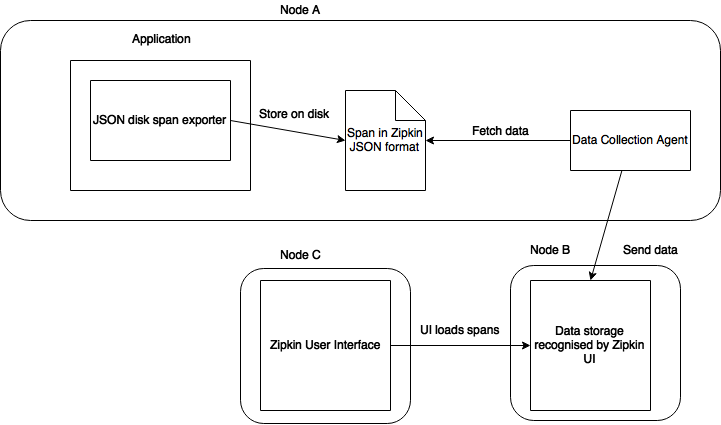
\includegraphics[scale=0.5]{disk_span_exporter.png}
		\caption{Using the JSON disk exporter together with the data collection service but Zipkin user interface .}
		\label{fig:disk_span_exporter}
	\end{figure}
\end{itemize}
Additionally, the Figure \ref{fig:custom_span_exporter} shows how a custom span exporter may be used.

\begin{figure}
	\centering
	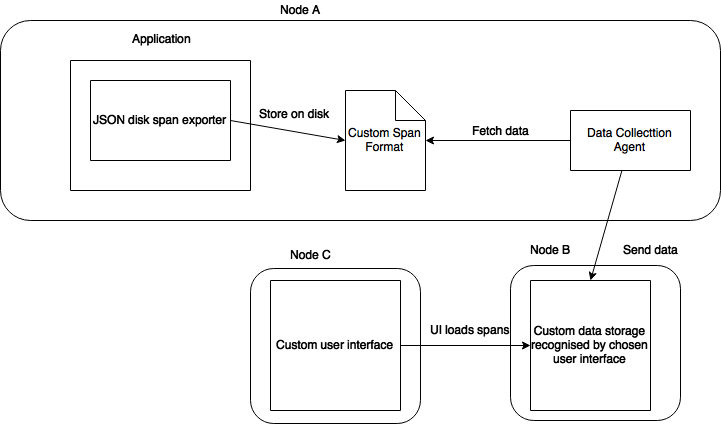
\includegraphics[scale=0.5]{custom_span_exporter.png}
	\caption{Using custom span exporter together with the data collection service and custom user interface.}
	\label{fig:custom_span_exporter}
\end{figure}
In order to give the developer the flexibility to add new exporters without changing the internals, the span exporters have to be  registered in the META-INF directory of the extended instrumentation server JAR file. This ensures that the service loader can find all implementations of the \texttt{SpanExporter} abstract class. The reason why the classes need to be discovered is explained in the following Section \ref{native_agent_design}

To make the developer life easier, the \textbf{AutoService} library\footnote{The AutoService library is available at \url{https://github.com/google}.} is used. Instead of manually registering the implemented span exporters into META-INF directory, they can be annotated in the code using the \texttt{AutoService} annotation with a single argument specifying the abstract parent, in this case \texttt{SpanExporter}. The library takes care of registering the classes automatically in the desired folder in correct format so the human error is minimized.
\section{Native Agent}
The native agent consists of several interesting technical parts. This section covers the instrumentation itself and also explains considered approaches during the development. The problem of instrumentation server requiring the dependencies for each instrumented class is explained together with the problem of instrumenting the classes with cyclic dependencies. The final solution is explain as well. 

In the following part, the internals of how JVM bytecode is parsed is explained.
\subsection{Instrumentation}
In general, the native agent does not perform the instrumentation but gets bytecode for the required class, sends the bytecode to the instrumentation server and applies the instrumented bytecode after receiving it from the client. 

The instrumentation server required all dependencies to be available for the currently instrumented class. This means that all other classes mentioned as part of method and field signatures, super classes or interfaces has to be available on the instrumentation server. To achieve this, two solutions have been tried but only the second solution shown to be feasible.

The first and unsuccessful solution was based on the fact that several on class file load hooks may be executed at several time in different threads. When the application loads a class, the class load hook event is triggered for it and its bytecode is made available. In this method, the new class file load hook event was artificially enforced via the \texttt{RetransformClasses} method. This method accepts array of classes for which the hook should be re-thrown. In order to continue with the instrumentation of the original class, all dependent classes have to be instrumented in this solution first. This also means that in this approach, the classes with cyclic dependencies are not supported. In order to instrumented such a class, all dependencies have to be instrumented first which is also the class itself.

This solution had also different problem. Since a number of dependencies can be significant, the problem of too many threads being opened at a single time has also appeared. 

The second and currently used solution is based on the fact that the Java class files may be accessed as a resource using the class loader of the class currently being load. Disadvantage of this solution that the developer may override the \texttt{getResourceAsStream} method on the custom class loader and not provide access to he class files. This is a limitation of the thesis. However, when a such event happens, the instrumentation does not end with the exception but first, the attempt to load the class using a different class loader is done. 

In this solution, the instrumentation server is first asked whether the current class should be instrumented based on the server's extensions. If the class is designed to be instrumented, its bytecode is send to the instrumentation server (only in case if the bytecode for the class is not already available). Then, dependencies are scanned via parsing the raw JVM bytecode which is explained in detail in the following section. Dependency loading is recursively called for each new dependent class until the class does not have any other dependencies or if all the dependencies are already uploaded to the instrumentation server. Once all dependencies for a class have been sent to the server, the instrumentation is invoked and the agent waits for the new bytecode. 

 Also several helper classes are sent back to the native agent at the stage where the class is checked whether it should be instrumented or not. The classes are auxiliary Byte Buddy classes and also instances of \texttt{LoadedTypeInitializer} class. The initializers are sent as serialized 
instances and therefore their defining class has to be available in the application. This is achieved in the agent initialization phase where several required classes are sent to the application from the server. The instances are saved to a map which maps the initializer name to its serialized representation. This initializer is later using during the class preparation phase to set the static interceptor field of the instrumented class as mentioned in the previous sections.

The auxiliary classes are classes created at run-time during the instrumentation on the server and have to be available on the applications machine as well. This is achieved by loading the bytecode for the auxiliary class, saving the class as a java class file on the disk and making it available by adding the class on the application's class path.

\subsection{Byte Code Parsing}
Byte code parsing is necessary feature of the thesis and is required in order to be able to get the list of dependent classes on a class currently being loaded. No sufficient C++ implementation has not been found and therefore a custom parsing module has been implemented. The parsing module is based on the Apache Commons BCEL Java package and the simplified version but still with the same logic has been rewritten to C++.

The main class used for parsing is \texttt{ClassParser} which contains \texttt{parse} method accepting the bytecode of a class and defines also several accessors  for the parsed data such as the super class name and complete reference, list of all implemented interfaces, list of all methods or list of all defined fields and their types.

The bytecode starts with the several important parts:
\begin{itemize}
	\item \textbf{Magic id}. Magic id is a first integer stored in each bytecode and contains  always 0xCAFEBABE number.
	\item \textbf{Version}. This part contains actually two shorts, where the first short represents minor Java version and the later one represents major Java version.
	\item \textbf{Constant pool}. Constant pool is a table representing class and interface names, field names and also other important constants. It contains mapping from id representing the type to the fully qualified type name.
	\item \textbf{Class Info}. Class information contains the information whether the bytecode represents a class or an interface, denotes class name and also super class name.
	\item \textbf{Interfaces}. This part contains the number of interfaces this class implements followed by id of type short of each interface. The interface can be looked up using the class pool.
	\item \textbf{Fields}. This part of the bytecode contains the number of fields this class defines together with some additional information for each defined field.
	\item \textbf{Methods}. This part contains the number of defined methods in the bytecode together wit additional information per each method such as the number of arguments.
\end{itemize}
More information about class file structure can be found at the official Java documentation\footnote{The documentation of the class loading process is available at \url{https://docs.oracle.com/javase/specs/jvms/se7/html/jvms-4.html}}.
Each part of the class file mentioned above is parsed separately. For accessing the raw bytecode a \texttt{ByteReader} class is used. It contains methods fro reading different types of data from the bytecode array. 

Parsing the magic id and both minor and major versions is straightforward as their are just numbers and can be read using the byte reader class directly. Parsing of the constant pool is more complex. For each entry in the constant pool a constant representing the entry is read. The constant can be of several type such as constant representing the Class symbol, String symbol, Method types of Field types for example. Once the Constant pool is parsed, it can be queried for the specific symbol by its id. Class name and super class name, interfaces, fields and methods are read from the constant pool by using their ids.

\section{Instrumentation Server Optimizations}
The instrumentation server does several optimizations to speed the communication with the native agent. The first optimization is caching of the classes sent to the instrumentation server from the native agent and also caching of the already instrumented classes. This behavior is useful in case we are using the shared instrumentation server. In this case multiple native agents are sharing the same instrumentation server. When a class is received from any agent, it is cached and the rest of the native agents don't need to send the original class again. The instrumentation server also performs the instrumentation only once and caches the instrumented class. When any agent requests to instrument already instrumented class on the server, the server just sends the class immediately from the cache.

The other way how the communication can be optimized can be influenced by the user. The user may compile the extended instrumentation server with the application classes or add these classes on the classpath of the server. When a native agent asks the server for instrumenting some class, the server first check if it can load the original class itself locally and avoid sending the bytecode from the native agent. 
\section{Span Injection on Instrumentation Server}
This short section explains how additional fields such as the span information are internally attached to the instrumented classes. The trace information is attached to the instrumented class by adding a new synthetic field with name \texttt{\_\_\_\_traceId}. This trace id represents the current trace and is used in the code to obtain reference to a current trace context and also current span.  A new field is created using the Byte Buddy instrumentation builder using the \texttt{defineField} method.
\section{Determine the Current Span Exporter}
This section explains how a span exporter type and also other arguments passed to the native agent are made accessible to the instrumentation server. The span exporter type is defined as part of the native agent and needs to be available at the instrumentation server as well. This is achieved by creating and registering the native method to a class, which is defined as part of the instrumentation server.
In case of span exporters, the abstract class \texttt{SpanExporter} is defined at the instrumentation server and contains native native method named \texttt{getSpanExporterType} for getting the span exporter type. The abstract \texttt{SpanExporter} class is sent to the native agent during the initialization phase. When this class is required for the first time, the native method implementation is bound to the method \texttt{getSpanExporterType} defined in the \texttt{SpanExporter} class. Therefore, even the classes defined as part of the instrumentation server can use methods defined on the native agent with really small overhead. Actually, there may be a performance gain, since these methods are written as native methods.



